\documentclass{article}
\usepackage{graphicx}
\usepackage{graphicx}
\usepackage{amssymb}
\usepackage{float}
\usepackage{amsmath}
\usepackage{algorithm}
\usepackage{algpseudocode}
\usepackage{indentfirst}

\title{Logistic Regression and Gradient Descent}
\author{ }
\date{ }

\begin{document}

	\maketitle

    Another type of learning algorithm is one based on optimization. In minimizing some function $J$, called an objective function, the learning algorithm should in effect minimize the training set error on $D_n$ of the classifier it produces. \\

    Objective function $J$ should be written as $J(\Theta) = {1\over{n}}{\sum^n_{i=1}}{L(h(x^{(i)}, \Theta),y^{(i)})+\lambda{R(\Theta)}}$. The first addend is the training set error of hypothesis $h$. The second addend is a new concept. $R(\Theta)$ is a regularizer. It prevents the learning algorithm from being too honed in on minimizing training set error. Sometimes, learning algorithms that are too focused on minimizing training set error produce a classifier that works too specifically well on training data that it is out of touch with the real-life data it will be thrown in the future. $\lambda$ is a positive constant (a hyperparameter) that determines to what degree the regularizer will be considered. Also, one must know that $\Theta$ is used to generally represent all parameters of $h$. For the scope of logistic regression, $\Theta$ encompasses $\theta$ and $\theta_0$. \\

    The type of hypothesis produced in linear regression is different from a standard linear classifier. The hypothesis in linear regression is written as $h(x; \theta, \theta_0)=\sigma(\theta^Tx+\theta_0)$ when $\sigma$ is the sigmoid function. The sigmoid function is defined as $\sigma(z)={{1}\over{1+e^{-z}}}$. Why can't one use a standard linear classifier and the zero-one loss function in the objective function to be optimized? Zero-one loss only says whether or not a separator classifies a point correctly or incorrectly. On the other hand, because $\sigma(z)\in(0,1)$ and $\sigma(0)=0.5$, the sigmoid function says how correctly or incorrectly a separator classifies a point. These semantics are what optimization takes advantage of in working towards the optimal set of parameters.

    \begin{figure}[H]
        \centering
        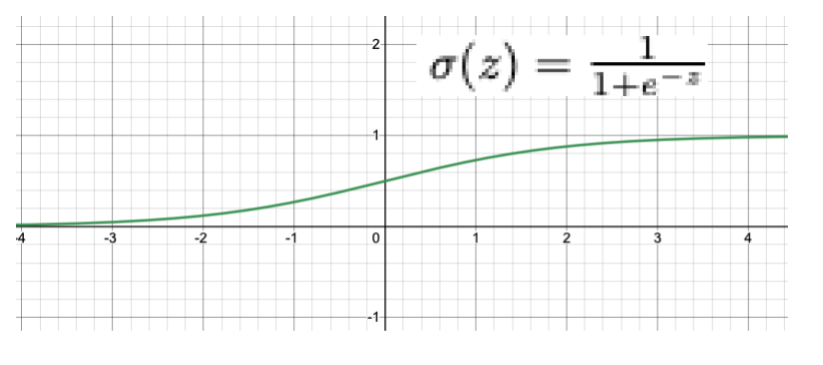
\includegraphics[width=0.5\linewidth]{Sigmoid Function.png}
    \end{figure}

    To actually classify points using $h(x; \theta, \theta_0)=\sigma(\theta^Tx+\theta_0)$ though, one needs to interpret the output of $\sigma$. For instance, if the threshold is 0.5, all outputs of $\sigma$ greater than 0.5 will be considered +1 whereas all outputs less than or equal to 0.5 will be negative. However, because the bounds of the sigmoid function's range are 0 and 1, $y^{(i)}\in{0,1}$ in the dataset. The most common setup is for the threshold to be 0.5. In that case, wherever $\sigma(z)=0.5$ is the linear classifier.

    \begin{figure}[H]
        \centering
        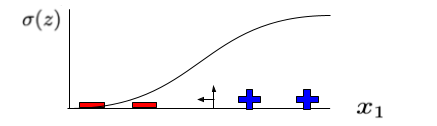
\includegraphics[width=0.5\linewidth]{Classifier Using Sigmoid Function.png}
    \end{figure}

    To visualize this phenomenon in the two dimensional space, imagine a plane curved like the sigmoid function sticking out through the third axis. The separator is where the sigmoid axis is 0.5.

    \section{Negative Log Likelihood Loss}
    The loss function that goes with the hypothesis logistic regression produces is called negative log likelihood loss. Deriving the function will allow one to make good sense of it.
        \begin{enumerate}
            \item The probability that $\theta$ and $\theta_0$ classify the dataset $D_n$ can be written as $\prod^n_{i=1}{\begin{cases}
                g^{(i)}, y^{(i)}=1\\
                1-g^{(i)} , y^{(i)}=0
            \end{cases}}=\prod^n_{i=1}({{g^{(i)}}^{y^{(i))}}+(1-g^{(i)})^{(1-y^{(i)})}})$.
            Each data point being classified is an independent event. Therefore, the probability of them all being classified correctly is the product of each point's probability of being correctly classified.

            \item Sums are easier to work with than products. Quite conveniently, the logarithm of a product is a sum. Also, because $\log{x}$ is monotonic, minimizing $\log{x}$ minimizes $x$. Thus, one should just work with $\log{(\prod^n_{i=1}({{g^{(i)}}^{y^{(i))}}+(1-g^{(i)})^{(1-y^{(i)})}})})$. Computing the logarithm produces $\sum^n_{i=1}({y^{(i)}\log{g^{(i)}}+(1-y^{(i)})\log{(1-g^{i})}})$.

            \item Even though the sum works for maximizing the probability that $\theta$ and $\theta_0$ classify the data, the job is still to design a loss functions. Loss functions should be minimized. The simple solution is negating the sum: $-\sum^n_{i=1}({y^{(i)}\log{g^{(i)}}+(1-y^{(i)})\log{(1-g^{i})}})$.

            \item The loss function will simply be the summand of the summation: $L(g,a)=-(a\log{g}+(1-a)\log{(1-g)})$.

        \end{enumerate}
    Negative log likelihood loss is also called cross entropy loss or log loss. \\

    \section{Regularizer}
    A common regularizer is $R(\Theta)=||\Theta||^2$. It tries to keep the norms of the parameters small during training. As a result, the learning algorithm will not try too hard to produce a classifier that does well on outlier points. The regularizer also prevents the classifier from overfitting the provided training data.

    \section{Learning Algorithm for Logistic Regression: Gradient Descent}
    Gradient descent is a common optimization learning algorithm for logistic regression. To understand how gradient descent works, one can begin by observing it in one dimension. \\

    Say there is some function $f$, some starting position called $x_{init}$, and some step size $\eta$. The algorithm obtains the derivative of $f$ at $x_{init}$. It then moves in the negative direction of the derivative. The size of the step it takes is determined by $\eta$. Eventually, after enough moving around, gradient descent should find a relative minimum of $f$. \\

    \begin{figure}[H]
        \centering
        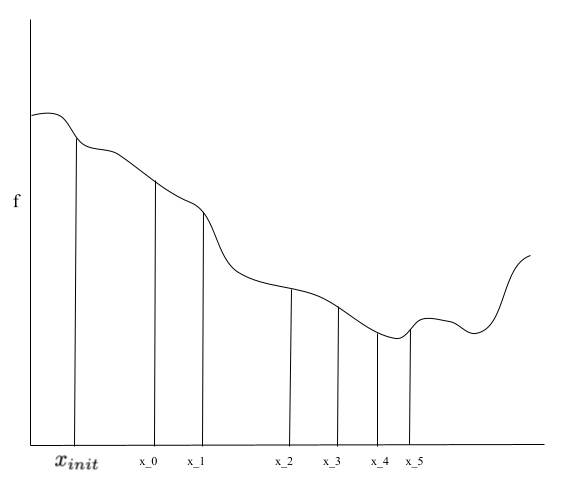
\includegraphics[width=0.5\linewidth]{Gradient Descent.png}
    \end{figure}

    In the figure above, $x$ will continue bouncing back and forth until its movements are less than some tolerance constant $\epsilon$.

    \section{Partial Derivatives and Gradients}
    Examine the multivariable function $f(x,y) = x^2y$. The partial derivative $\frac{\partial{x}}{\partial{f}}$ is the derivative of $x^2y$ when y is treated like a constant. The same is true for $\frac{\partial{y}}{\partial{f}}$, except $x$ is treated like a constant. Neither partial derivative tells the entire rate of change of $f$, but they do give insight into how $f$ changes as one of its variables does. The gradient of $f$, written as $\nabla{f}$ is the vector of all partial derivatives of $f$:
        $\begin{bmatrix}
               \frac{\partial{x}}{\partial{f}} \\
               \frac{\partial{y}}{\partial{f}} \\
        \end{bmatrix}$.

    \section{Gradient Descent in Multiple Dimensions}
    \begin{algorithm}
    \begin{algorithmic}[]
        \State \textbf{Input:} $\theta_{init}$, $f$, $\nabla_\theta{f}$, $\epsilon$, $\eta$
        \State $\theta^{(0)} = \theta_{init}$
        \State $t=0$
        \While{$f(\theta^{(t)})-f(\theta^{(t-1)})\geq \epsilon$}
            \State $t = t+1$
            \State $\theta^{(t)}=\theta^{(t-1)}-\eta{\nabla{f(\theta^{(t-1)})}}$
        \EndWhile \\
        \Return $\theta$
    \end{algorithmic}
    \end{algorithm}

    \section{Gradient Descent for Logistic Regression}
    Gradient descent for logistic regression uses the listed formulas. \\
    $J(\theta, \theta_0) = {1\over{n}}{\sum_{i=1}^n{L(\sigma(\theta^Tx+\theta_0),y^{(i)})}+\frac{\lambda}{2}{||\theta||^2}}$. \\
    $\nabla_\theta{J(\theta, \theta_0)}=\frac{1}{n}\sum_{i=1}^{n}{(\sigma(\theta^Tx+\theta_0),y^{(i)})-y^{(i)})x^{(i)}}+\lambda\theta$\\
    $\frac{\partial J(\theta, \theta_0)}{\partial \theta_0}={1\over{n}}\sum^n_{i=1}({\sigma(\theta^Tx+\theta_0)}-y^{(i)})$ \\
    The algorithm is the same, but the edits are the subtraction of the gradient above and the partial derivative above from $\theta_{(t)}$ and $\theta_0^{(t)}$ inside the loop.


\end{document}
